\chapter{Core concepts}
\label{chap:Core concepts}

In this chapter, we introduce the core concepts of the library. There are five
of them. At the center is a class that represent the state space, that is the
value of the states $\{X_t^i\}_{i=1}^{N_t}$. This class may also contain other
members that is specific for the model, such as the data. Next is the weights
$\{W_t^i\}_{i=1}^{N_t}$. Together with the states, they form a particle system.
A sampler operates on a particle system to produce samples iteratively. A
sampler might also use some monitors to calculate some estimates
$\varphi(\{X_t^i,W_t^i\}_{i=1}^{N_t})$ as it progresses. These concepts are all
abstracted in the library. For brevity, in the following we will drop the time
dependent index $t$.

\section{State}
\label{sec:State}

Let $E$ be the state space, a state object represents the states collection
$\{X^i\}_{i=1}^N$ and everything it depends on. If there exists $d\ge1$ and
some space $\calX$ such that $E\subseteq\calX^d$. Then, we can represent the
states as an $N$ by $d$ matrix. The element at row $i$ and column $j$ is thus
the $j$\ith component of $X^i$. In this situation, the library provides a
default implementation,
\begin{Verbatim}
  template <
      MatrixLayout Layout,
      std::size_t Dim,
      typename ValueType>
  class StateMatrix;
\end{Verbatim}
where \verb|Layout| is either \verb|RowMajor| or \verb|ColMajor|, which
specifies the matrix layout, \verb|Dim| is the dimension of $X$, i.e., $d$ and
\verb|ValueType| shall be a \cpp type that represents values in $\calX$. For
example, if $E\subseteq\Real^d$, then one can use the following class,
\begin{Verbatim}
  StateMatrix<RowMajor, d, double> state(N);
\end{Verbatim}
This is not a general purpose matrix class for use such as linear algebra. It
is more of a container with a few additional methods. Below is some common
operations can be done on \verb|state|,
\begin{Verbatim}
  state.size();          // Get the sample size
  state.dim();           // Get the dimension
  state.resize(N);       // Change the sample size
  state(i, j);           // The element at row i, column j
  state.at(i, j);        // Same as above but with assertion
\end{Verbatim}
If the template parameter \verb|Dim| is equal to zero, then it is assumed that
the dimension is dynamic and may change later. In this case, there are
additional methods,
\begin{Verbatim}
  StateMatrix<RowMajor, Dynamic, double> state(N, d);
  state.resize(N, d);  // Change the sample size and dimension
  state.resize_dim(d); // Change the dimension
\end{Verbatim}
The enumerator \verb|Dynamic| above has the value zero. Note that, these
methods are only available when the template parameter \verb|Dim| is zero.
Attempting to call these methods when it is positive will result in
compile-time errors. Let $p$ be the minimum of the original and new sample
sizes, and $q$ be the minimum of the original and new dimensions. All the
methods that change the size of the matrix will preserve the $p$ by $q$ matrix
at the upper left corner of the original.

It is also possible to get pointers to the raw data,
\begin{Verbatim}
  state.data();       // Equivalent to &state(0, 0)
  state.row_data(i);  // Equivalent to &state(i, 0)
  state.col_data(i);  // Equivalent to &state(0, j)
  state.row_stride(); // &state(i, j + 1) - &state(i, j)
  state.col_stride(); // &state(i + 1, j) - &state(i, j)
\end{Verbatim}
These pointer can provide either read only or read and write access to the raw
data, depends on if the \verb|state| object is constant. Note that, the stride
of the pointer returned by \verb|row_data| and \verb|col_data| depends on the
template parameter \verb|Layout|. Therefore, to iterate over a specific row,
\begin{Verbatim}
  auto rowptr = state.row_data(i);
  auto stride = state.row_stride();
  for (size_type j = 0; j != state.dim(); ++j, rowptr += stride)
      /* *rowptr is the as state(i, j) */; 
\end{Verbatim}
And similarly, to iterate over a specific column,
\begin{Verbatim}
  auto colptr = state.col_data(j);
  auto stride = state.col_stride();
  for (size_type i = 0; i != state.dim(); ++i, colptr += stride)
      /* *colptr is the as state(i, j) */; 
\end{Verbatim}
One can also retrieve a whole row or column through an output iterator. For
example, to read the column $1$ and $3$ into a vector,
\begin{Verbatim}
  std::vector<ValueType> col13(state.size() * 2);
  auto first = col13.begin();
  first = state.read_col(1, first);
  first = state.read_col(3, first);
\end{Verbatim}
There is a similar \verb|read_row| method. To read the whole matrix into a
vector,
\begin{Verbatim}
  std::vector<ValueType> matrix(state.size() * state.dim());
  state.read(RowMajor, matrix.begin());
\end{Verbatim}
The first parameter is matrix layout of the output matrix. There are two more
methods, whose purpose will become clear later. The first is,
\begin{Verbatim}
  void duplicate(size_type src, size_type dst);
\end{Verbatim}
Let the value of \verb|src| and \verb|dst| be $p$ and $q$, respectively. This
method set the value of $X^p$ to that of $X^q$. In other words, $X^p$ is
duplicated while $X^q$ is eliminated. The other method is,
\begin{Verbatim}
  template <typename IntType, typename InputIter>
  void select(IntType N, InputIter index);
\end{Verbatim}
where \verb|index| is an $N$-vector, say $\{a_i\}_{i=1}^N$. This method select
samples to form a new collection $\{\hat{X}^i\}_{i=1}^N$ such that $\hat{X}^i =
X^{a_i}$. The sample size $N$ does not have to be the same as the original, say
$M$. This is closely related to the selection step of \smc algorithms. Let $r_i
= \sum_{j = 1}^N\bbI_{\{i\}}(a_j)$. Then it is required that $a_i = i$ for all
$r_i > 0$, $i = 1,\dots,\min\{N, M\}$.

\section{Weight}
\label{sec:Weight}

The weights $\{W^i\}_{i=1}^N$ is abstracted by the class \verb|Weight|. For
example,
\begin{Verbatim}
  Weight w(N);
  w.size();    // Get the sample size
  w.resize(N); // Change the sample size
\end{Verbatim}
One important property of \verb|Weight| is that, $\{W^i\}_{i=1}^N$ is always
normalized. For example, after the construction or resizing, the weights are
set to be equal, i.e., $W^i = 1 / N$, for $i = 1,\dots,N$. One can manually set
the weights to be equal by,
\begin{Verbatim}
  w.set_equal();
\end{Verbatim}
The weights can be manipulated in various way. Let \verb|v| be an input
iterator pointing to an $N$-vector $\{v^i\}_{i=1}^N$. To set $W^i \propto v^i$,
use
\begin{Verbatim}
  w.set(v);
\end{Verbatim}
To set $\log W^i = v^i + \mathrm{constant}$, use
\begin{Verbatim}
  w.set_log(v);
\end{Verbatim}
To set weights incrementally, use
\begin{Verbatim}
  w.mul(v);
  w.add_log(v);
\end{Verbatim}
which sets $W^i \propto W^i v^i$ and $\log W^i = \log W^i + v^i +
\mathrm{constant}$, respectively. The value of \ess of the weights can be
obtained by,
\begin{Verbatim}
  w.ess();
\end{Verbatim}
One may also draw an integer $0 \le k < N$ according to the weights by,
\begin{Verbatim}
  w.draw(rng);
\end{Verbatim}
where \verb|rng| is a \cppoo{} \rng engine object. Last, one can obtain a
pointer to the raw data,
\begin{Verbatim}
  w.data();
\end{Verbatim}
or read all the weights into an output iterator,
\begin{Verbatim}
  w.read(first);
\end{Verbatim}
Unlike \verb|StateMatrix|, the pointer returned by the \verb|data| method
always provides read only access. In other words, \verb|Weight| does not
provide any means for user to change an individual $W^i$ without changing the
others. Conceptually, it is the relative weights that matter. And changing one
of them is in fact changing $\{W^i\}_{i=1}^N$ as a whole.

\section{Particle}
\label{sec:Particle}

A particle system, abstracted by the class template,
\begin{Verbatim}
  template <typename T>
  class Particle;
\end{Verbatim}
is essentially formed by three parts. The first is an object of type \verb|T|,
that abstracts the states $\{X^i\}_{i=1}^N$. The second is a type \verb|Weight|
object that abstracts the weights $\{W^i\}_{i=1}^N$. And the third is a
collection of \cppoo{} \rng engines. There are some restrictions on the type
\verb|T|. The constructor of \verb|Particle| is as the following,
\begin{Verbatim}
  template <typename... Args>
  explicit Particle(size_type N, Args &&... args)
\end{Verbatim}
where the first argument is the sample size. This and all other arguments, are
passed down to the constructor of type \verb|T|. For example,
\begin{Verbatim}
  using T = StateMatrix<RowMajor, Dynamic, double>;
  Particle<T> particle(N, d);
\end{Verbatim}
will construct the \verb|StateMatrix| object with arguments \verb|N| and
\verb|d|. Therefore, \verb|T| must has a constructor that accepts an integer
value as its first argument. The acceptable additional arguments of the
constructor of \verb|Particle| is the same as those of \verb|T|. Second,
\verb|T| has to provide a \verb|select| method similar to that of
\verb|StateMatrix|. The library does not impose any restriction on the internal
structure of \verb|T|. And thus it cannot perform the selection by itself.
However, for more complicated situations, one can always define a class, say
\verb|ValueType| to represent the space $E$, and use a one dimension
\verb|StateMatrix| as the type \verb|T|. For example,
\begin{Verbatim}
  class ValueType; // User defined type
  using T = StateMatrix<RowMajor, 1, ValueType>;
  Particle<T> particle(N);
\end{Verbatim}
More usefully, one can create a new type by deriving from \verb|StateMatrix|.
Note that, though the \verb|select| method of \verb|StateMatrix| is written as
a function template that can accept any integers and input iterators as its
arguments, the user defined type \verb|T| only need to support the following
signature,
\begin{Verbatim}
  ReturnType select(size_type N, const size_type *index);
\end{Verbatim}
where \verb|size_type| is \verb|T::size_type| if such a type exists, and
\verb|std::size_t| otherwise.

The \verb|Weight| type object is constructed with a single argument, the sample
size $N$. To retrieve references to the type \verb|T| and \verb|Weight|
objects, one can call,
\begin{Verbatim}
  particle.state();
  particle.weight();
\end{Verbatim}
respectively. Last but not least, the \verb|Particle| class also contains a
collection of \rng engines. The method,
\begin{Verbatim}
  particle.rng(i);
\end{Verbatim}
returns a reference to an \rng engine, specific to the $i$\ith particle. For $i
\ne j$, if the following,
\begin{Verbatim}
  auto &rng_i = particle.rng(i);
  auto &rng_j = particle.rng(j);
\end{Verbatim}
are called from two different threads, then \verb|rng_i| and \verb|rng_j| will
be instances of two independent \rng engines. The details are in
Section~\ref{sec:Multiple RNG streams}. The \verb|Particle| class also contains
an \rng engine independent of any particle,
\begin{Verbatim}
  auto &rng = particle.rng();
\end{Verbatim}
We will revisit this topic later when we discuss multi-threaded implementations
in the next chapter.

\subsection{Resize the particle system}
\label{sub:Resize the particle system}

The sample size of a particle system can be obtained by,
\begin{Verbatim}
  particle.size();
\end{Verbatim}
It can be changed. However, in Monte Carlo algorithms, one does not change the
sample size arbitrarily. Which samples to be preserved and possibly duplicated
and which samples to be eliminated, has to be done according to some algorithms
that produce desirable effects. There are a few methods to resize a particle
system. They share two common properties. They take the new sample size, say
$N$, as their first argument. The other is that in the end, they call the
\verb|select| method on the type \verb|T| object, with $N$ and an input
iterator, say \verb|index|, that points to an $N$-vector $\{a_i\}_{i=1}^N$ as
arguments. In addition they all call the \verb|resize| method on the type
\verb|Weight| object with $N$ as the argument. How the type \verb|T| handles
the call to the \verb|select| method is up to the user. But usually it should
behave similarly to that of \verb|StateMatrix|. Below is descriptions of each
method for resizing a particle system. They differ in how they generate the
index vector $\{a_i\}_{i=1}^N$. We will let $M$ denote the original sample
size. Also, for clarity, in the mathematical description of the vectors, we are
using indices starting with $1$, while in the actual \cpp program, the indices
starts with zero, as usual.

\subsubsection{Resize with given index vectors}

\begin{Verbatim}
  template <typename InputIter>
  void resize_by_index(size_type N, InputIter index);
\end{Verbatim}
This method takes the index vector as its input and passes it directly to the
\verb|select| method of \verb|T|.

\subsubsection{Resize with resampling algorithms}

\begin{Verbatim}
  template <typename ResampleType>
  void resize_by_resample(size_type N, ResampleType &&res)
\end{Verbatim}
This method generates the index vector according to a resampling algorithm. A
resampling algorithm produce the number of replications of each particle in the
original system. The function \verb|res| shall accept a call as the following,
\begin{Verbatim}
  res(M, N, rng, w, r);
\end{Verbatim}
where $M$ and $N$ are the original and new sample size, \verb|rng| is a
reference to an \rng engine, \verb|w| is a pointer of type \verb|double|, that
points to the $M$-vector of normalized weights. And last, \verb|r| is a pointer
of type \verb|size_type| that points to the $M$-vector of the number of
duplicates of each particles $\{r_i\}_{i=1}^M$. It is required that, the
results shall satisfy $r_i\ge0$ for $i=1,\dots,M$ and $\sum_{i=1}^M r_i = N$.
The index vector is generated such that,
\begin{gather*}
  a_i = i \text{ if } r_i > 0 \text{ for } i = 1,\dots,\min\{N, M\} \\
  \sum_{i=1}^N\bbI_{\{j\}}(a_i) = r_j \text{ for } j = 1,\dots,M
\end{gather*}

\subsubsection{Resize with uniform selection}

\begin{Verbatim}
  void resize_by_uniform(size_type N);
\end{Verbatim}
The index vector is generated such that, $\Prob(a_i = j) = 1/M$, for $i =
1,\dots,N$, $j = 1,\dots,M$. This is equivalent to Multinomial resampling with
equal weights.

\subsection{Clone the particle system}
\label{sub:Clone the particle system}

The \verb|Particle<T>| class has the usual special members, such as the copy
constructor, assignment operator, etc. They work just as usual. For example,
\begin{Verbatim}
  auto new_particle = particle;
\end{Verbatim}
This creates a new particle system as an exact duplicate of the original.
However, this ``exactness'' is often undesired. The duplicated particle system
will have exactly the same states of \rng engines as the original. And
therefore, any random samples generated from this new system will be exactly
the same as the original. This is hardly the desired effects in algorithms
where duplicating a particle system into multiple copies is required. In this
situation, one can use the \verb|clone| method,
\begin{Verbatim}
  auto new_particle = particle.clone();
\end{Verbatim}
In contrast to the copy constructor, this will create a new particle system
exactly the same as the original, except that all \rng engines within the new
system is re-seeded.

\subsection{Iterate the particle system}
\label{sub:Iterate the particle system}

As mentioned before, the library does not impose restrictions on how the states
shall be structured or accessed. Therefore it is not possible to access $X^i$
using methods of \verb|Particle|. Instead, one has to use methods of \verb|T|,
the type of the template parameter. For example,
\begin{Verbatim}
  using T = StateMatrix<RowMajor, d, double>;
  Particle<T> particle(N);
  particle.state()(i, j);
  particle.state().dim();
\end{Verbatim}
This is rather cumbersome and somehow too limited. The library provides a class
template,
\begin{Verbatim}
  template <typename T>
  class ParticleIndex;
\end{Verbatim}
that represents the index of particles within the system. It is constructed by
the index of the particle and a pointer to the particle system that it belongs
to. For example,
\begin{Verbatim}
  ParticleIndex<T> idx(i, &particle);
\end{Verbatim}
or alternatively,
\begin{Verbatim}
  auto idx = particle.index(i);
\end{Verbatim}
To access the particle system, use
\begin{Verbatim}
  idx.particle();     // A reference to particle
  idx.particle_ptr(); // A pointer to particle
\end{Verbatim}
For any type \verb|T|, the type \verb|ParticleIndex<T>| has the following
methods,
\begin{Verbatim}
  idx.i();   // The index used to construct idx, i
  idx.rng(); // => particle.rng(i);
\end{Verbatim}
If \verb|T| is a derived class of \verb|StateMatrix|, then
\begin{Verbatim}
  idx.dim();    // => particle.state().dim();
  idx.stride(); // => particle.state().row_stride();
  idx.data();   // => particle.state().row_data(i);
  idx(j);       // => particle.state()(i, j);
  idx.at(j);    // => particle.state().at(i, j);
\end{Verbatim}
That is, \verb|ParticleIndex| has an interface that depends on the type
\verb|T|. One can extend its interface by defining a special member class
template inside \verb|T|. For example,
\begin{Verbatim}
  using Base = StateMatrix<RowMajor, d, double>;

  class T : public Base
  {
      public:
      template <typename S>
      using idx_base = Base::particle_index_type<S>;

      template <typename S>
      class particle_index_type : public idx_base<S>
      {
          public:
          particle_index_type(size_type i, Particle<S> *pptr) :
              idx_base<S>(i, pptr)
          {
          }
      };
  };
\end{Verbatim}
The class \verb|ParticleIndex<T>| derives from \verb|T::particle_index_type<T>|
if such a member class template exists. Otherwise, it has methods as described
earlier for any type \verb|T|. Therefore, it is possible to give
\verb|ParticleIndex<T>| methods that are more convenient for a particular
problem. We will see examples later in Section~\ref{sec:Example (PF)}.

The \verb|ParticleIndex| type can also be used like an random access iterator.
For example,
\begin{Verbatim}
  auto idx = particle(i);
  auto jdx = particle(j);
  ++idx;      // => particle.index(i + 1);
  idx--;      // => particle.index(i - 1);
  idx + n;    // => particle.index(i + n);
  idx - jdx;  // => i - j;
  idx == jdx; // => i == j;
\end{Verbatim}
Other comparison operators such as \verb|!=|, \verb|<|, etc., are also
defined. Note that, comparing or subtracting two indices from two different
particles systems is meaningless. This will result in runtime errors unless
debugging is disabled (see Section~\appref{sec:Error handling}). The increment
and decrement operators follow usual \cpp prefix and postfix semantics.
However, it is important to note that, \verb|ParticleIndex| \emph{is not} an
iterator even though it shares many common methods. Recall that,
\verb|Particle| does not have methods to access $X^i$ directly. And therefore
it is not possible to dereference a \verb|ParticleIndex| object to get a
reference to $X^i$. Instead, dereferencing an \verb|ParticleIndex| object will
return a reference to itself. This is similar for the member access operator
and the index operator. For example,
\begin{Verbatim}
  *idx;       // => idx
  idx->rng(); // => idx.rng();
  idx[n];     // => idx + n
\end{Verbatim}
These methods may at first seem pointless. However, it makes it possible to
iterate a \verb|Particle| object. For example,
\begin{Verbatim}
  for (auto idx : particle) {
      idx(0) = /* initialize the first dimension */;
      idx(1) = /* initialize the second dimension */;
      // ...
  }
\end{Verbatim}
This is equivalent to
\begin{Verbatim}
  for (size_t i = 0; i != particle.size(); ++i) {
      auto idx = particle.index(i);
      // ...
  }
\end{Verbatim}
More importantly, it allows the use of \verb|Particle| with algorithms. For
example,
\begin{Verbatim}
  auto s = std::accumulate(particle.begin(), particle.end(), 0.0,
      [](double s, ParticleIndex<T> idx) { return s + idx(0); });
\end{Verbatim}

\section{Sampler}
\label{sec:Sampler}

A sampler is formed by the particle system together with all the operations on
it. It is abstracted by the class template,
\begin{Verbatim}
  template <typename T>
  class Sampler;
\end{Verbatim}
The template parameter \verb|T| is the same as that of \verb|Particle|. Its
constructor takes arbitrary arguments,
\begin{Verbatim}
  template <typename... Args>
  explicit Sampler(Args &&... args)
\end{Verbatim}
and all arguments are passed down to the constructor of \verb|Particle|. For
example,
\begin{Verbatim}
  using T = StateMatrix<RowMajor, Dynamic, double>;
  Sampler<T> sampler(N, d);
\end{Verbatim}
Any callable objects that is convertible to the following can be used as
operations on the particle system,
\begin{Verbatim}
  using eval_type = std::function<void(
      std::size_t,
      Particle<T> &)>;
\end{Verbatim}
For example,
\begin{Verbatim}
  void eval(std::size_t iter, Particle<T> &particle);
\end{Verbatim}
Conceptually, such a function implement an operator $M(\{X^i,W^i\}_{i=1}^N)$
such that a new particle system $\{\hat{X}^i,\hat{W}^i\}_{i=1}^{\hat{N}}$ is
produced given the original. It it often possible to decompose the operator $M$
into multiple simpler ones. And thus a sampler can have a sequence of
evaluation objects. Each of these evaluation objects can be added to the
sampler by the \verb|eval| method,
\begin{Verbatim}
  Sampler<T> &eval(
      const eval_type &new_eval,
      SamplerStage stage);
\end{Verbatim}
For example,
\begin{Verbatim}
  sampler.eval(eval, SamplerInit | SamplerMove, true);
\end{Verbatim}
The first argument is the evaluation object. The sampler maintains a sequence
of evaluation steps. The new evaluation object will be appended to the existing
sequence. Note that, the order at which these objects being evaluated is the
same as the one they are added to the sampler. One can clear the sequence by,
\begin{Verbatim}
  sampler.eval_clear();
\end{Verbatim}
The second argument will be explained shortly. The sampler can also have an
optional resampling step. This can be added to the sampler by the following
method,
\begin{Verbatim}
  Sampler<T> &resample_method(
      ResampleScheme scheme,
      double threshold = resample_threshold_always());
\end{Verbatim}
which uses a builtin resampling scheme of the library (see
Section~\ref{sec:Builtin algorithms}). Or alternatively,
\begin{Verbatim}
  Sampler<T> &resample_method(
      const eval_type &res_eval,
      double threshold = resample_threshold_always());
\end{Verbatim}
In either case, the parameter \verb|threshold| specifies the condition under
which the resampling step will be actually performed. Let its value be
$\alpha$, resampling is performed if and only if $\ess < \alpha N$.

\subsection{Evaluation stages}
\label{sub:Evaluation stages}

The sampler is iterated with two methods,
\begin{Verbatim}
  sampler.initialize();
  sampler.iterate(n);
\end{Verbatim}
The first initialize the sampler, and the second iterate the sampler $n$ times.
In each case, the sequence of user defined evaluation objects will be called,
such as the \verb|eval| function defined earlier. The first argument passed to
it is the iteration number. This number is reset to zero when \verb|initialize|
is called and incremented by one each time the sampler is iterated. The
initialization is divided into the following stages,
\begin{description}
  \item[\texttt{SamplerInit}] Initialize $\{X_0^i,W_0^i\}_{i=1}^{N_0}$.
  \item[Resampling] If $\ess < \alpha N$, resample to
    $\{\hat{X}_0^i,\hat{W}_0^i\}_{i=1}^{\hat{N}_0}$.
  \item[\texttt{SamplerMCMC}] Mutate to
    $\{\check{X}_0^i,\check{W}_0^i\}_{i=1}^{\check{N}_0}$.
\end{description}
For $t\ge1$, the iteration at time $t$, is divided into the following stages,
\begin{description}
  \item[\texttt{SamplerMove}] Move from
    $\{\check{X}_{t-1}^i,\check{W}_{t-1}^i\}_{i=1}^{\check{N}_{t-1}}$ to
    $\{X_t^i,W_t^i\}_{i=1}^{N_t}$.
  \item[Resampling] If $\ess < \alpha N$, resample to
    $\{\hat{X}_t^i,\hat{W}_t^i\}_{i=1}^{\hat{N}_t}$.
  \item[\texttt{SamplerMCMC}] Mutate to
    $\{\check{X}_t^i,\check{W}_t^i\}_{i=1}^{\check{N}_t}$.
\end{description}
In each of these stages, one or more \verb|eval_type| objects are called upon
to perform the necessary sampling and calculation. In the \emph{Resampling}
stage, the evaluation object set by \verb|resmaple_method| will be used to
perform the resampling. The builtin algorithms will use the \verb|select|
method of the state type \verb|T| to perform the selection after generating the
index vector. In all other three types of stages, all objects in the sequence
of evaluation objects set by the \verb|eval| method of \verb|Sampler| is
checked. Recall that, each evaluation object is added to the sampler by a call
to the following method,
\begin{Verbatim}
  Sampler<T> &eval(
      const eval_type &new_eval,
      SamplerStage stage);
\end{Verbatim}
At each stage, the value of the second parameter will be checked. For example,
at the \verb|SamplerInit| stage, this object will be called if and only if the
value of \verb|(SamplerInit & stage)| is non-zero. The other two stages,
\verb|SamplerMove| and \verb|SamplerMCMC| is similar. The last one is so named
because in many algorithms, the mutation step is performed by some \mcmc
kernel. It is not universally so. Clearly, the evaluation objects at that
stage, if any, do not have to perform \mcmc type mutations. To give a more
concrete example, lets consider the following,
\begin{Verbatim}
  sampler.eval(eval1, SamplerInit);
  sampler.eval(eval2, SamplerMove);
  sampler.eval(eval3, SamplerInit | SamplerMove);
  sampler.eval(eval4, SamplerMCMC);
  sampler.resample_method(Multinomial);
\end{Verbatim}
Then when the following is called,
\begin{Verbatim}
  sampler.initialize().iterate(n);
\end{Verbatim}
The algorithm performed is as the following,
\begin{enumerate}
  \item Initialize once
    \begin{enumerate}
      \item Set $t \leftarrow 0$
      \item Apply \verb|eval1|
      \item Apply \verb|eval3|
      \item Apply resampling
      \item Apply \verb|eval4|
    \end{enumerate}
  \item Iterate $n$ times
    \begin{enumerate}
      \item Set $t \leftarrow t + 1$
      \item Apply \verb|eval2|
      \item Apply \verb|eval3|
      \item Apply resampling
      \item Apply \verb|eval4|
    \end{enumerate}
\end{enumerate}
Note that, \verb|eval3| is applied in both the initialization and iteration
steps.

\section{Monitor}
\label{sec:Monitor}

Let $\varphi_t(\{X_t^i,W_t^i\}_{i=1}^{N_t})$ be some estimator with values in
$\Real^d$. It is often of interest to monitor its value as the algorithm
progresses. In the library, this is done through the class template
\verb|Monitor|. It has the following constructor,
\begin{Verbatim}
  Monitor(
      std::size_t dim,
      const eval_type &eval,
      bool record_only = false,
      MonitorStage stage = MonitorMCMC);
\end{Verbatim}
The first parameter \verb|dim| is the dimension of $\varphi_t$, $d$. The second
is a user defined callback function. More specifically,
\begin{Verbatim}
  using eval_type = std::function<void(
      std::size_t,
      std::size_t,
      Particle<T> &,
      double *)>;
\end{Verbatim}
For example,
\begin{Verbatim}
  void varphi(
      std::size_t t,
      std::size_t d,
      Particle<T> &particle,
      double *r);
\end{Verbatim}
When this function is called. The first argument passed to it is $t$, the
iteration number. The second is $d$, the dimension. The third is a reference to
the particle system at iteration $t$. And the last is a pointer to a vector for
output.

The third parameter of the constructor of \verb|Monitor|, \verb|record_only|
determines how shall the function above behave. If it is true, then the
function \verb|varphi| shall return the value of $\varphi_t$ directly, and the
output parameter \verb|r| points to a $d$-vector. In this case, \verb|Monitor|
merely records the values of $\varphi_t$ at each iteration. On the other hand,
if \verb|record_only| is false, then it is assumed that $\varphi_t$ takes the
following form,
\begin{equation*}
  \varphi_t(\{X_t^i,W_t^i\}_{i=1}^{N_t}) =
  \sum_{i=1}^{N_t} W_t^i \varphi_t^i(X_t^i).
\end{equation*}
And the output parameter \verb|r| is an $N$ by $d$ row major matrix, with the
$d$-vector value $\varphi_t^i(X_t^i)$ written into each row of this matrix. And
each time \verb|varphi| is called, \verb|Monitor| will compute and store the
result of the summation above.

The last parameter of the constructor of \verb|Monitor| specifies when shall
the calculation of $\varphi_t$ be carried out. Possible values are,
\begin{description}
  \item[\texttt{MonitorMove}] Evaluate after the \verb|SamplerInit| or
    \verb|SamplerMove| stages and right before the possible resampling.
  \item[\texttt{MonitorResample}] Evaluate right after the possible
    \emph{Resampling} stage.
  \item[\texttt{MonitorMCMC}] Evaluate after the \verb|SamplerMCMC| stage,
    i.e., at the end of the initialization or iteration.
\end{description}

A monitor can be added to a sampler. For example,
\begin{Verbatim}
  Monitor<T> mon(d, eval, false, MonitorMCMC);
  sampler.monitor("name", mon);
\end{Verbatim}
If a monitor with the same name already exists, then the old one will be
removed, and the new one will be appended to the end of the monitoring
sequence. Note that, the order at which the monitors being evaluated is the
same as the one they are added to the sampler. This ordering is of importance
if a monitor alternate the particle system in any way, which is allowed even
though unusual. A new monitor with the same name does not take the place of the
old one.

Monitors can be retrieved by,
\begin{Verbatim}
  const auto &mon = sampler.monitor("name");
\end{Verbatim}
One can also remove the monitor from the sampler by,
\begin{Verbatim}
  sampler.monitor_clear("name");
\end{Verbatim}
or remove all monitors by,
\begin{Verbatim}
  sampler.monitor_clear();
\end{Verbatim}
One can retrieve the results in various ways. Every time a monitor being
evaluated, it records two values. The first is the iteration number $t$, at
which it was evaluated. The other is the value of $\varphi_t$. One can retrieve
these values using the following methods,
\begin{Verbatim}
  mon.iter_size();  // Total number of evaluations
  mon.index(j);     // Iteration number of the j-th evaluation
  mon.record(i, j); // The value of the i-th component
                    // of the result at the j-th evaluation
\end{Verbatim}
Note that, the monitor does not have to be added to a sampler before it
starting initialization. It can also be removed before the sampler finishing
all iterations. Therefore, the iteration numbers of a monitor being evaluated
are not necessarily the sequence $0,1,\dots,n$, where $n$ is the total number
of iterations.

\section{Example}
\label{sec:Example (PF)}

This is an example used in \textcite{Johansen:2009wd}. Through this example, we
will show how to implement a simple particle filter. It shall walk one through
the basic features of the library introduced above.

\subsection{Model and algorithm}
\label{sub:Model and algorithm}

The state space model, known as the almost constant velocity model in the
tracking literature, provides a simple scenario. The state vector,
\begin{equation*}
  X_t = (\xpos^t, \ypos^t, \xvel^t, \yvel^t)^{\transpose}
\end{equation*}
contains the position and velocity of an object moving in a plane. Imperfect
observations $Y_t = (\xobs^t, \yobs^t)^{\transpose}$ of the positions are
possible at each time instance. The state and observation equations are linear
with additive noises,
\begin{align*}
  X_t &= AX_{t-1} + V_t \\
  Y_t &= BX_t + \delta W_t
\end{align*}
where
\begin{equation*}
  A = \begin{pmatrix}
    1 & 0 & \Delta & 0      \\
    0 & 1 & 0      & \Delta \\
    0 & 0 & 1      & 0      \\
    0 & 0 & 0      & 1
  \end{pmatrix} \qquad
  B = \begin{pmatrix}
    1 & 0 & 0 & 0 \\
    0 & 1 & 0 & 0 \\
  \end{pmatrix} \qquad
  \delta = 0.1
\end{equation*}
and we assume that the elements of the noise vector $V_t$ are independent
Gaussian with variance $0.02$ and $0.001$ for position and velocity,
respectively. The observation noise, $W_t$ comprises i.i.d.\ $t$-distributed
random variables with degree of freedom $\nu = 10$. The prior at time $0$
corresponds to an axis-aligned Gaussian with variance $4$ for the position
coordinates and $1$ for the velocity coordinates. The particle filter algorithm
is shown in Algorithm~\ref{alg:pf}.

\begin{algorithm}[t]
  \begin{algorithmic}
    \hrule\vskip1ex
    \STATE \emph{Initialization}
    \STATE\STATESKIP Set $t\leftarrow0$.
    \STATE\STATESKIP Sample
    $\xpos^{0,i},\ypos^{0,i}\sim\calN(0,4)$ and
    $\xvel^{0,i},\yvel^{0,i}\sim\calN(0,1)$.
    \STATE\STATESKIP Weight $W_0^i \propto \exp\{\ell(X_0^i|Y_0)\}$
    where $\ell$ is the log-likelihood function.

    \STATE \emph{Iteration}
    \STATE\STATESKIP Set $t\leftarrow t + 1$.
    \STATE\STATESKIP Sample
    \begin{align*}
      \xpos^{t,i}&\sim\calN(\xpos^{t-1,i} + \Delta\xvel^{t-1,i}, 0.02) &
      \xvel^{t,i}&\sim\calN(\xvel^{t-1,i}, 0.001) \\
      \ypos^{t,i}&\sim\calN(\ypos^{t-1,i} + \Delta\yvel^{t-1,i}, 0.02) &
      \yvel^{t,i}&\sim\calN(\yvel^{t-1,i}, 0.001)
    \end{align*}
    \STATE\STATESKIP Weight $W_t^i \propto W_{t-1}^i\exp\{\ell(X_t^i|Y_t)\}$.

    \STATE \emph{Repeat the \emph{Iteration} step until all data are processed}.
    \vskip1ex\hrule
  \end{algorithmic}
  \caption{Particle filter for the almost constant velocity model}
  \label{alg:pf}
\end{algorithm}

\subsection{Implementation}
\label{sub:Implementation (PF)}

We will work through a complete implementation using a top-down approach.
First, we show the \verb|main| function.
\begin{Verbatim}
  int main()
  {
      const std::size_t N = 1000;

      Sampler<PF> sampler(N);

      sampler.resample_method(Stratified, 0.5)
          .eval(PFInit, SamplerInit)
          .eval(PFMove, SamplerMove)
          .eval(PFWeight, SamplerInit | SamplerMove)
          .monitor("pos", Monitor<PF>(2, PFEstimate));

      sampler.initialize();
      sampler.iterate(sampler.particle().state().n() - 1);

      std::ofstream out("pf.out");
      out << sampler;
      out.close();

      return 0;
  }
\end{Verbatim}
In a real application, the sample size $N$ is likely to be determined by some
user input. For brevity, we simply used a constant here. Within the \verb|main|
function, a \verb|Sampler| object is first constructed with the specified
number of particles. Then we configure the sampler. First, it will use
stratified resampling when $\ess < N / 2$. The sampling step within the
\emph{Initialization} and \emph{Iteration} in Algorithm~\ref{alg:pf} will be
implemented by two functions, \verb|PFInit| and \verb|PFMove|, respectively.
The weighting is done through the function \verb|PFWeight|. And the estimate
will be monitored through the function \verb|PFEstimate|. These are added to
the sampler through the \verb|eval| and \verb|monitor| methods as shown above.
After configuring the sampler, we initialize it and iterate $n - 1$ times,
where $n$ is the total number of observations, including at time $t = 0$. In
the end, we write a summary of the sampler into the file \verb|pf.out|. This
\verb|main| function is a simple translation of the algorithm described
earlier. Now we show the details of the implementation each function used.

\subsubsection{The \texttt{PF} class}

First all of, we need a class to represent the state space, which is $\Real^4$.
A sensible base class is thus,
\begin{Verbatim}
  using PFBase = StateMatrix<RowMajor, 4, double>;
\end{Verbatim}
The class \verb|PF| is declared as below,
\begin{Verbatim}
  class PF : public PFBase
  {
      public:
      template <typename T>
      class particle_index_type;

      PF(std::size_t N);
      std::size_t n() const { return obs_x_.size(); };

      private:
      std::vector<double> obs_x_;
      std::vector<double> obs_y_;
  };
\end{Verbatim}
The constructor will initialize the observations,
\begin{Verbatim}
  PF(std::size_t N) : PFBase(N)
  {
      double x = 0;
      double y = 0;
      std::ifstream data("pf_cv.data");
      while (data >> x >> y) {
          obs_x_.push_back(x);
          obs_y_.push_back(y);
      }
      data.close();
  }
\end{Verbatim}
Again, in a real application, the data is unlikely to be initialized in this
way. The method \verb|n| simply return the size of \verb|obs_x_|. Last, we
would like to extend the \verb|ParticleIndex<PF>| class, by defining the member
class template \verb|particle_index_type|,
\begin{Verbatim}
  template <typename T>
  using PFIndexBase = PFBase::particle_index_type<T>;

  template <typename T>
  class particle_index_type : public PFIndexBase<T>
  {
      public:
      particle_index_type(std::size_t i, Particle<T> *pptr)
          : PFIndexBase<T>(i, pptr)
      {
      }

      double &pos_x() { return this->at(0); }
      double &pos_y() { return this->at(1); }
      double &vel_x() { return this->at(2); }
      double &vel_y() { return this->at(3); }

      double log_likelihood(std::size_t iter);
  }; // class particle_index_type
\end{Verbatim}
First of all, we don't want to later refer to the states $\xpos$, etc., by
integer index values in the reset of the program, which is error prone even for
this simple example. Second, we would like to compute the log-likelihood of any
given particle. This is implemented through the \verb|log_likelihood| method,
which is a simple translation of the mathematical formulation,
\begin{Verbatim}
  double log_likelihood(std::size_t iter)
  {
      const double x = this->particle().state().obs_x_[iter];
      const double y = this->particle().state().obs_y_[iter];
      const double scale = 10;
      const double nu = 10;

      double llh_x = scale * (pos_x() - x);
      double llh_y = scale * (pos_y() - y);
      llh_x = std::log(1 + llh_x * llh_x / nu);
      llh_y = std::log(1 + llh_y * llh_y / nu);

      return -0.5 * (nu + 1) * (llh_x + llh_y);
  }
\end{Verbatim}

\subsubsection{The \texttt{PFInit} and \texttt{PFMove} functions}

The function that sample the state values from the prior is as the following,
\begin{Verbatim}
  inline void PFInit(std::size_t, Particle<PF> &particle)
  {
      std::normal_distribution<double> rpos(0, 2);
      std::normal_distribution<double> rvel(0, 1);
      auto &rng = particle.rng();

      for (auto idx : particle) {
          idx.pos_x() = rpos(rng);
          idx.pos_y() = rpos(rng);
          idx.vel_x() = rvel(rng);
          idx.vel_y() = rvel(rng);
      }
  }
\end{Verbatim}
We construct two Normal distribution objects using for the position and
velocity components of the states. And initialize each particle with them. The
function to sample new states in each iteration later is similar,
\begin{Verbatim}
  inline void PFMove(std::size_t, Particle<PF> &particle)
  {
      std::normal_distribution<double> rpos(0, std::sqrt(0.02));
      std::normal_distribution<double> rvel(0, std::sqrt(0.001));
      auto &rng = particle.rng();
      const double delta = 0.1;

      for (auto idx : particle) {
          idx.pos_x() += rpos(rng) + delta * idx.vel_x();
          idx.pos_y() += rpos(rng) + delta * idx.vel_y();
          idx.vel_x() += rvel(rng);
          idx.vel_y() += rvel(rng);
      }
  }
\end{Verbatim}
Both of these two functions are really simple translations of the mathematical
formulation of the algorithm.

\subsubsection{The \texttt{PFWeight} function}

In each iteration, we will weight the particles using its log-likelihood. This
will be computed with the \verb|log_likelihood| method of
\verb|particle_index_type| defined earlier,
\begin{Verbatim}
  inline void PFWeight(std::size_t iter, Particle<PF> &particle)
  {
      std::vector<double> weight(particle.size());
      for (auto idx : particle)
          weight[idx.i()] = idx.log_likelihood(iter);
      particle.weight().add_log(weight.data());
  }
\end{Verbatim}
The last step in the function above add the logarithm of the incremental
weights to the particle system. Note that, each time the \verb|initialize|
method of \verb|Sampler| is called, the weights will be set to be equal first.
And thus the function above is correct for both initialization and iterations.

\subsubsection{The \texttt{PFEstimate} function}

Last, we would like to record the value of $\varphi_t(X_t^i) =
(\xpos^{t,i},\ypos^{t,i})^{\transpose}$. This is done by defining the function,
\begin{Verbatim}
  inline void PFEstimate(
      std::size_t,
      std::size_t,
      Particle<PF>
      &particle,
      double *r)
  {
      for (auto idx : particle) {
          *r++ = idx.pos_x();
          *r++ = idx.pos_y();
      }
  }
\end{Verbatim}
The out parameter \verb|r| points to an $N$ by $d$ row major matrix, $d = 2$.

\subsubsection{Summary}

As we see above, the implementation of all the functions added to the sampler
object is straightforward. In fact, half of the program is within the
definition of the \verb|PF| class. This is in fact a common pattern of programs
using this library. The class that represent the state space also contains
methods and data that is specific to the model.

The first few lines of the output of the program, written by
\begin{Verbatim}
  std::ofstream out("pf.out");
  out << sampler;
  out.close();
\end{Verbatim}
is shown below
\begin{Verbatim}
  ESS   Resampled       Size    pos.0   pos.1
  2.13795       1       1000    -1.29499        3.11821
  357.471       1       1000    -1.22486        3.18716
  152.535       1       1000    -1.31156        2.99123
\end{Verbatim}
One can read this text file into a statistical program, for exmaple
R\footnote{\url{http://r-project.org}}, to produce Figure~\ref{fig:pf}. More
advanced methods for saving summaries and histories of a sampler is given in
Section~\ref{sec:Store objects in HDF5 format}, using the \hdf format.

\begin{figure}
  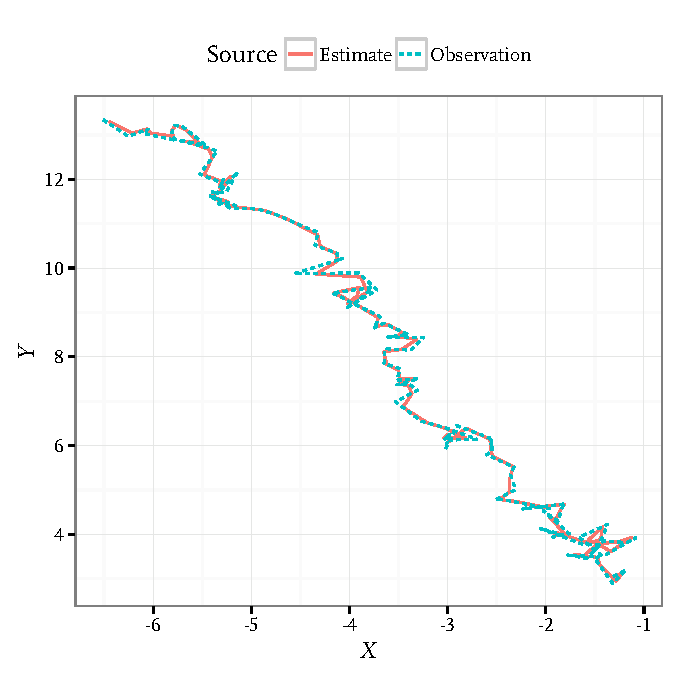
\includegraphics{fig/pf}
  \caption{Estimates and observations of the particle filter}
  \label{fig:pf}
\end{figure}
